% Options for packages loaded elsewhere
\PassOptionsToPackage{unicode}{hyperref}
\PassOptionsToPackage{hyphens}{url}
\PassOptionsToPackage{dvipsnames,svgnames,x11names}{xcolor}
\PassOptionsToPackage{space}{xeCJK}
%
\documentclass[
  9pt,
  a4paper,
  ignorenonframetext,
  notheorems]{beamer}
\usepackage{pgfpages}
\setbeamertemplate{caption}[numbered]
\setbeamertemplate{caption label separator}{: }
\setbeamercolor{caption name}{fg=normal text.fg}
\beamertemplatenavigationsymbolshorizontal
% Prevent slide breaks in the middle of a paragraph
\widowpenalties 1 10000
\raggedbottom
\setbeamertemplate{part page}{
  \centering
  \begin{beamercolorbox}[sep=16pt,center]{part title}
    \usebeamerfont{part title}\insertpart\par
  \end{beamercolorbox}
}
\setbeamertemplate{section page}{
  \centering
  \begin{beamercolorbox}[sep=12pt,center]{part title}
    \usebeamerfont{section title}\insertsection\par
  \end{beamercolorbox}
}
\setbeamertemplate{subsection page}{
  \centering
  \begin{beamercolorbox}[sep=8pt,center]{part title}
    \usebeamerfont{subsection title}\insertsubsection\par
  \end{beamercolorbox}
}
\AtBeginPart{
  \frame{\partpage}
}
\AtBeginSection{
  \ifbibliography
  \else
    \frame{\sectionpage}
  \fi
}
\AtBeginSubsection{
  \frame{\subsectionpage}
}

\usepackage{amsmath,amssymb}
\usepackage{iftex}
\ifPDFTeX
  \usepackage[T1]{fontenc}
  \usepackage[utf8]{inputenc}
  \usepackage{textcomp} % provide euro and other symbols
\else % if luatex or xetex
  \usepackage{unicode-math}
  \defaultfontfeatures{Scale=MatchLowercase}
  \defaultfontfeatures[\rmfamily]{Ligatures=TeX,Scale=1}
\fi
\usepackage{lmodern}
\usetheme[outer/progressbar=foot,outer/numbering=fraction,inner/sectionpage=none]{metropolis}
\usecolortheme{seahorse}
\usefonttheme{metropolis}
\usefonttheme{serif} % use mainfont rather than sansfont for slide text
\useoutertheme{metropolis}
\ifPDFTeX\else  
    % xetex/luatex font selection
  \setmainfont[]{HelveticaNeue}
  \setsansfont[]{Fira Mono}
  \setmonofont[Scale=0.75,Color=orange]{Fira Mono}
  \ifXeTeX
    \usepackage{xeCJK}
    \setCJKmainfont[]{NanumGothic}
          \fi
  \ifLuaTeX
    \usepackage[]{luatexja-fontspec}
    \setmainjfont[]{NanumGothic}
  \fi
\fi
% Use upquote if available, for straight quotes in verbatim environments
\IfFileExists{upquote.sty}{\usepackage{upquote}}{}
\IfFileExists{microtype.sty}{% use microtype if available
  \usepackage[]{microtype}
  \UseMicrotypeSet[protrusion]{basicmath} % disable protrusion for tt fonts
}{}
\makeatletter
\@ifundefined{KOMAClassName}{% if non-KOMA class
  \IfFileExists{parskip.sty}{%
    \usepackage{parskip}
  }{% else
    \setlength{\parindent}{0pt}
    \setlength{\parskip}{6pt plus 2pt minus 1pt}}
}{% if KOMA class
  \KOMAoptions{parskip=half}}
\makeatother
\usepackage{xcolor}
\geometry{lmargin=.2in,rmargin=.2in,bmargin=.4in}
\newif\ifbibliography
\setlength{\emergencystretch}{3em} % prevent overfull lines
\setcounter{secnumdepth}{-\maxdimen} % remove section numbering

\usepackage{color}
\usepackage{fancyvrb}
\newcommand{\VerbBar}{|}
\newcommand{\VERB}{\Verb[commandchars=\\\{\}]}
\DefineVerbatimEnvironment{Highlighting}{Verbatim}{commandchars=\\\{\}}
% Add ',fontsize=\small' for more characters per line
\usepackage{framed}
\definecolor{shadecolor}{RGB}{241,243,245}
\newenvironment{Shaded}{\begin{snugshade}}{\end{snugshade}}
\newcommand{\AlertTok}[1]{\textcolor[rgb]{0.68,0.00,0.00}{#1}}
\newcommand{\AnnotationTok}[1]{\textcolor[rgb]{0.37,0.37,0.37}{#1}}
\newcommand{\AttributeTok}[1]{\textcolor[rgb]{0.40,0.45,0.13}{#1}}
\newcommand{\BaseNTok}[1]{\textcolor[rgb]{0.68,0.00,0.00}{#1}}
\newcommand{\BuiltInTok}[1]{\textcolor[rgb]{0.00,0.23,0.31}{#1}}
\newcommand{\CharTok}[1]{\textcolor[rgb]{0.13,0.47,0.30}{#1}}
\newcommand{\CommentTok}[1]{\textcolor[rgb]{0.37,0.37,0.37}{#1}}
\newcommand{\CommentVarTok}[1]{\textcolor[rgb]{0.37,0.37,0.37}{\textit{#1}}}
\newcommand{\ConstantTok}[1]{\textcolor[rgb]{0.56,0.35,0.01}{#1}}
\newcommand{\ControlFlowTok}[1]{\textcolor[rgb]{0.00,0.23,0.31}{#1}}
\newcommand{\DataTypeTok}[1]{\textcolor[rgb]{0.68,0.00,0.00}{#1}}
\newcommand{\DecValTok}[1]{\textcolor[rgb]{0.68,0.00,0.00}{#1}}
\newcommand{\DocumentationTok}[1]{\textcolor[rgb]{0.37,0.37,0.37}{\textit{#1}}}
\newcommand{\ErrorTok}[1]{\textcolor[rgb]{0.68,0.00,0.00}{#1}}
\newcommand{\ExtensionTok}[1]{\textcolor[rgb]{0.00,0.23,0.31}{#1}}
\newcommand{\FloatTok}[1]{\textcolor[rgb]{0.68,0.00,0.00}{#1}}
\newcommand{\FunctionTok}[1]{\textcolor[rgb]{0.28,0.35,0.67}{#1}}
\newcommand{\ImportTok}[1]{\textcolor[rgb]{0.00,0.46,0.62}{#1}}
\newcommand{\InformationTok}[1]{\textcolor[rgb]{0.37,0.37,0.37}{#1}}
\newcommand{\KeywordTok}[1]{\textcolor[rgb]{0.00,0.23,0.31}{#1}}
\newcommand{\NormalTok}[1]{\textcolor[rgb]{0.00,0.23,0.31}{#1}}
\newcommand{\OperatorTok}[1]{\textcolor[rgb]{0.37,0.37,0.37}{#1}}
\newcommand{\OtherTok}[1]{\textcolor[rgb]{0.00,0.23,0.31}{#1}}
\newcommand{\PreprocessorTok}[1]{\textcolor[rgb]{0.68,0.00,0.00}{#1}}
\newcommand{\RegionMarkerTok}[1]{\textcolor[rgb]{0.00,0.23,0.31}{#1}}
\newcommand{\SpecialCharTok}[1]{\textcolor[rgb]{0.37,0.37,0.37}{#1}}
\newcommand{\SpecialStringTok}[1]{\textcolor[rgb]{0.13,0.47,0.30}{#1}}
\newcommand{\StringTok}[1]{\textcolor[rgb]{0.13,0.47,0.30}{#1}}
\newcommand{\VariableTok}[1]{\textcolor[rgb]{0.07,0.07,0.07}{#1}}
\newcommand{\VerbatimStringTok}[1]{\textcolor[rgb]{0.13,0.47,0.30}{#1}}
\newcommand{\WarningTok}[1]{\textcolor[rgb]{0.37,0.37,0.37}{\textit{#1}}}

\providecommand{\tightlist}{%
  \setlength{\itemsep}{0pt}\setlength{\parskip}{0pt}}\usepackage{longtable,booktabs,array}
\usepackage{calc} % for calculating minipage widths
\usepackage{caption}
% Make caption package work with longtable
\makeatletter
\def\fnum@table{\tablename~\thetable}
\makeatother
\usepackage{graphicx}
\makeatletter
\def\maxwidth{\ifdim\Gin@nat@width>\linewidth\linewidth\else\Gin@nat@width\fi}
\def\maxheight{\ifdim\Gin@nat@height>\textheight\textheight\else\Gin@nat@height\fi}
\makeatother
% Scale images if necessary, so that they will not overflow the page
% margins by default, and it is still possible to overwrite the defaults
% using explicit options in \includegraphics[width, height, ...]{}
\setkeys{Gin}{width=\maxwidth,height=\maxheight,keepaspectratio}
% Set default figure placement to htbp
\makeatletter
\def\fps@figure{htbp}
\makeatother

\RequirePackage{fontspec} \RequirePackage{calc} \RequirePackage{microtype} \RequirePackage{etoolbox} \RequirePackage{chngcntr} \RequirePackage{scrextend} \RequirePackage{contour} \RequirePackage[normalem]{ulem} \RequirePackage{underscore} \RequirePackage{hyperref} \titlegraphic{
\includegraphics[width=4cm]{images/hanyang.png}} \definecolor{hyublue}{HTML}{0E4A84} \definecolor{hyulightblue}{HTML}{6e92b5} \definecolor{hyusilver}{HTML}{898C8E} \definecolor{hyulightsilver}{HTML}{6a737b} \setbeamercolor{title}{fg=hyublue} \setbeamercolor{frametitle}{bg=hyusilver!25, fg=hyublue} \setbeamercolor{background canvas}{bg=White} \setbeamercolor{block title}{bg=white, fg=hyublue} \setbeamercolor{block body}{bg=white} \setbeamercolor{block title example}{bg=hyulightblue, fg=white} \setbeamercolor{block body example}{bg=hyulightblue!25} \setbeamercolor{progress bar}{fg=hyulightblue} \setbeamertemplate{blocks}[rounded][shadow=false] \setbeamerfont{title}{size=\fontsize{20}{20}} \setbeamerfont{frametitle}{size=\fontsize{14}{20}} %\setbeamerfont{title}{family=\fontfamily{montserrat}\selectfont} \setlength{\leftmargini}{5pt} % set bullet left margin \setlength{\leftmarginii}{5pt}
\makeatletter
\makeatother
\makeatletter
\makeatother
\makeatletter
\@ifpackageloaded{caption}{}{\usepackage{caption}}
\AtBeginDocument{%
\ifdefined\contentsname
  \renewcommand*\contentsname{Table of contents}
\else
  \newcommand\contentsname{Table of contents}
\fi
\ifdefined\listfigurename
  \renewcommand*\listfigurename{List of Figures}
\else
  \newcommand\listfigurename{List of Figures}
\fi
\ifdefined\listtablename
  \renewcommand*\listtablename{List of Tables}
\else
  \newcommand\listtablename{List of Tables}
\fi
\ifdefined\figurename
  \renewcommand*\figurename{Figure}
\else
  \newcommand\figurename{Figure}
\fi
\ifdefined\tablename
  \renewcommand*\tablename{Table}
\else
  \newcommand\tablename{Table}
\fi
}
\@ifpackageloaded{float}{}{\usepackage{float}}
\floatstyle{ruled}
\@ifundefined{c@chapter}{\newfloat{codelisting}{h}{lop}}{\newfloat{codelisting}{h}{lop}[chapter]}
\floatname{codelisting}{Listing}
\newcommand*\listoflistings{\listof{codelisting}{List of Listings}}
\makeatother
\makeatletter
\@ifpackageloaded{caption}{}{\usepackage{caption}}
\@ifpackageloaded{subcaption}{}{\usepackage{subcaption}}
\makeatother
\makeatletter
\@ifpackageloaded{tcolorbox}{}{\usepackage[skins,breakable]{tcolorbox}}
\makeatother
\makeatletter
\@ifundefined{shadecolor}{\definecolor{shadecolor}{rgb}{.97, .97, .97}}
\makeatother
\makeatletter
\makeatother
\makeatletter
\makeatother
\ifLuaTeX
  \usepackage{selnolig}  % disable illegal ligatures
\fi
\IfFileExists{bookmark.sty}{\usepackage{bookmark}}{\usepackage{hyperref}}
\IfFileExists{xurl.sty}{\usepackage{xurl}}{} % add URL line breaks if available
\urlstyle{same} % disable monospaced font for URLs
\hypersetup{
  pdftitle={Introduction to the R language (2)},
  pdfauthor={Seoncheol Park},
  colorlinks=true,
  linkcolor={hyublue},
  filecolor={hyublue},
  citecolor={hyublue},
  urlcolor={hyublue},
  pdfcreator={LaTeX via pandoc}}

\title{Introduction to the R language (2)}
\author{Seoncheol Park}
\date{}

\begin{document}
\frame{\titlepage}
\ifdefined\Shaded\renewenvironment{Shaded}{\begin{tcolorbox}[boxrule=0pt, enhanced, frame hidden, interior hidden, borderline west={3pt}{0pt}{shadecolor}, breakable, sharp corners]}{\end{tcolorbox}}\fi

\begin{frame}[fragile]{2.5 Packages, libraries, and repositories}
\protect\hypertarget{packages-libraries-and-repositories}{}
\begin{itemize}
\item
  We have already mentioned several \emph{packages}, i.e.~\texttt{base},
  \texttt{knitr}, and \texttt{chron}.
\item
  In R, a package is a module containing functions, data, and
  documentation.

  \begin{itemize}
  \tightlist
  \item
    R always contains the base packages (e.g.~\texttt{base},
    \texttt{stats}, \texttt{graphics}); these contain things that
    everyone will use.
  \item
    There are also contributed packages (e.g.~\texttt{knitr} and
    \texttt{chron}); these are modules written by others to use in R.
  \end{itemize}
\item
  When you start your R session, you will have some packages loaded and
  available for use, while others are stored on your computer in a
  \texttt{library}. To be sure a package is loaded, run code like
\end{itemize}

\begin{Shaded}
\begin{Highlighting}[]
\FunctionTok{library}\NormalTok{(knitr)}
\end{Highlighting}
\end{Shaded}

To see which packages are loaded, run

\begin{Shaded}
\begin{Highlighting}[]
\FunctionTok{search}\NormalTok{() }\CommentTok{\# Your list will likely be different from ours.}
\end{Highlighting}
\end{Shaded}

\begin{verbatim}
 [1] ".GlobalEnv"        "package:knitr"     "package:stats"    
 [4] "package:graphics"  "package:grDevices" "package:datasets" 
 [7] "renv:shims"        "package:utils"     "package:methods"  
[10] "Autoloads"         "package:base"     
\end{verbatim}
\end{frame}

\begin{frame}[fragile]
\begin{itemize}
\item
  \textbf{(WARNING)} A package can only contain one function of any
  given name, but the same name may be used in another package.
\item
  When you use that function, R will choose it from the first package in
  the search list.
\item
  you want to force a function to be chosen from a particular package,
  prefix the name of the function with the name of the package and
  \texttt{::}, e.g.
\end{itemize}

\begin{Shaded}
\begin{Highlighting}[]
\NormalTok{stats}\SpecialCharTok{::}\FunctionTok{median}\NormalTok{(x)}
\end{Highlighting}
\end{Shaded}

\begin{itemize}
\tightlist
\item
  If you try to use a package which is not installed on your computer,
  you will receive an error message:
\end{itemize}

\begin{Shaded}
\begin{Highlighting}[]
\FunctionTok{library}\NormalTok{(notInstalled)}
\end{Highlighting}
\end{Shaded}

\begin{verbatim}
Error in library(notInstalled): there is no package called 'notInstalled'
\end{verbatim}

\begin{itemize}
\tightlist
\item
  The biggest \textbf{repository} of R packages is known as
  \href{https://cran.r-project.orghttps://cran.r-project.org}{CRAN}. To
  install a package from CRAN, you can run a command like
\end{itemize}

\begin{Shaded}
\begin{Highlighting}[]
\FunctionTok{install.packages}\NormalTok{(}\StringTok{"knitr"}\NormalTok{)}
\end{Highlighting}
\end{Shaded}

or, within RStudio, click on the \texttt{Packages} tab in the Output
Pane, choose \texttt{Install}, and enter the name in the resulting
dialog box.
\end{frame}

\begin{frame}[fragile]{2.6.1 Help pages}
\protect\hypertarget{help-pages}{}
\begin{itemize}
\tightlist
\item
  If you know the name of the function that you need help with, the
  \texttt{help()} function is likely sufficient.

  \begin{itemize}
  \tightlist
  \item
    It may be called with a string or function name as an argument, or
  \item
    you can simply put a question mark (\texttt{?}) in front of your
    query.
  \end{itemize}
\item
  For example, for help on the \texttt{q()} function, type
\end{itemize}

\begin{Shaded}
\begin{Highlighting}[]
\NormalTok{?q }\CommentTok{\#or}
\FunctionTok{help}\NormalTok{(q)}
\end{Highlighting}
\end{Shaded}

or just hit the F1 key while pointing at q in RStudio. Any of these will
open a help page containing a description of the function for quitting
R.

\begin{itemize}
\tightlist
\item
  \texttt{help(mean)} tells us that \texttt{mean()} will compute the
  ordinary arithmetic average.
\end{itemize}

\begin{Shaded}
\begin{Highlighting}[]
\FunctionTok{help}\NormalTok{(mean)}
\end{Highlighting}
\end{Shaded}
\end{frame}

\begin{frame}[fragile]
\begin{itemize}
\tightlist
\item
  \texttt{help.search()} or `??{}`` are often used, when you don't know
  the function name.
\end{itemize}

\begin{Shaded}
\begin{Highlighting}[]
\NormalTok{??optimization}
\CommentTok{\#or}
\FunctionTok{help.search}\NormalTok{(}\StringTok{"optimization"}\NormalTok{)}
\end{Highlighting}
\end{Shaded}

\begin{itemize}
\tightlist
\item
  You may find pages describing functions that you do not have
  installed, because they are in user-contributed packages. You can
  usually install them by typing
\end{itemize}

\begin{Shaded}
\begin{Highlighting}[]
\FunctionTok{install.packages}\NormalTok{(}\StringTok{"packagename"}\NormalTok{)}
\end{Highlighting}
\end{Shaded}
\end{frame}

\begin{frame}[fragile]{2.6.2 Built-in examples}
\protect\hypertarget{built-in-examples}{}
\begin{itemize}
\tightlist
\item
  A useful supplement to \texttt{help()} is the \texttt{example()}
  function, which runs examples from the end of the help page:
\end{itemize}

\begin{Shaded}
\begin{Highlighting}[]
\FunctionTok{example}\NormalTok{(mean)}
\end{Highlighting}
\end{Shaded}

\begin{verbatim}

mean> x <- c(0:10, 50)

mean> xm <- mean(x)

mean> c(xm, mean(x, trim = 0.10))
[1] 8.75 5.50
\end{verbatim}

\begin{itemize}
\item
  These examples show simple use of the \texttt{mean()} function as well
  as how to use the \texttt{trim} argument.
\item
  When \texttt{trim\ =\ 0.1}, the highest 10\% and lowest 10\% of the
  data are deleted before the average is calculated.
\end{itemize}
\end{frame}

\begin{frame}[fragile]{2.7.1 Some built-in graphics functions}
\protect\hypertarget{some-built-in-graphics-functions}{}
\begin{itemize}
\tightlist
\item
  Two basic plots are the histogram and the scatterplot. The codes below
  were used to produce example graphs:
\end{itemize}

\begin{Shaded}
\begin{Highlighting}[]
\FunctionTok{hist}\NormalTok{(islands)}
\end{Highlighting}
\end{Shaded}

\begin{figure}

{\centering 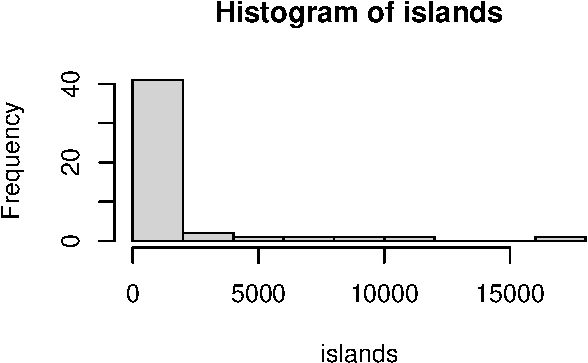
\includegraphics{03_introR02_files/figure-beamer/unnamed-chunk-13-1.pdf}

}

\end{figure}
\end{frame}

\begin{frame}[fragile]
\begin{Shaded}
\begin{Highlighting}[]
\NormalTok{x }\OtherTok{\textless{}{-}} \FunctionTok{seq}\NormalTok{(}\DecValTok{1}\NormalTok{, }\DecValTok{10}\NormalTok{) }
\NormalTok{y }\OtherTok{\textless{}{-}}\NormalTok{ x}\SpecialCharTok{\^{}}\DecValTok{2} \SpecialCharTok{{-}} \DecValTok{10} \SpecialCharTok{*}\NormalTok{ x }
\FunctionTok{plot}\NormalTok{(x, y)}
\end{Highlighting}
\end{Shaded}

\begin{figure}

{\centering 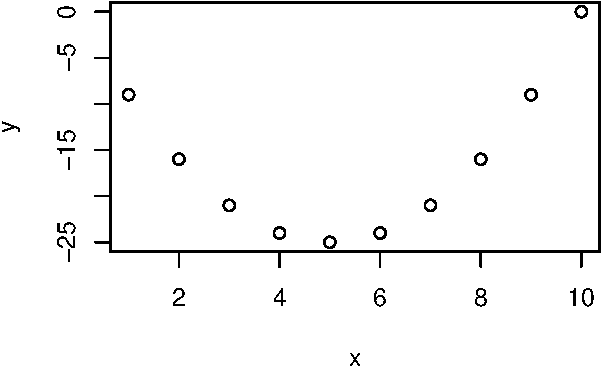
\includegraphics{03_introR02_files/figure-beamer/unnamed-chunk-14-1.pdf}

}

\end{figure}

Note that the \texttt{x} values are plotted along the horizontal axis.
\end{frame}

\begin{frame}[fragile]
\begin{itemize}
\tightlist
\item
  Another useful plotting function is the \texttt{curve()} function for
  plotting the graph of a univariate mathematical function on an
  interval.
\end{itemize}

\begin{Shaded}
\begin{Highlighting}[]
\CommentTok{\#plotting a sine function on [0,6pi]}
\FunctionTok{curve}\NormalTok{(}\AttributeTok{expr =}\NormalTok{ sin, }\AttributeTok{from =} \DecValTok{0}\NormalTok{, }\AttributeTok{to =} \DecValTok{6} \SpecialCharTok{*}\NormalTok{ pi)}
\end{Highlighting}
\end{Shaded}

\begin{figure}

{\centering 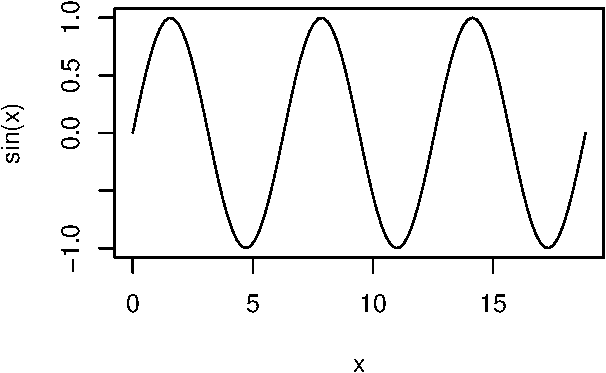
\includegraphics{03_introR02_files/figure-beamer/unnamed-chunk-15-1.pdf}

}

\end{figure}
\end{frame}

\begin{frame}[fragile]
\begin{itemize}
\tightlist
\item
  Note that the \texttt{expr} parameter is either a function (whose
  output is a numeric vector when the input is a numeric vector) or an
  expression in terms of \texttt{x}. An example of the latter type of
  usage is:
\end{itemize}

\begin{Shaded}
\begin{Highlighting}[]
\FunctionTok{curve}\NormalTok{(}\AttributeTok{expr =}\NormalTok{ x}\SpecialCharTok{\^{}}\DecValTok{2} \SpecialCharTok{{-}} \DecValTok{10} \SpecialCharTok{*}\NormalTok{ x, }\AttributeTok{from =} \DecValTok{1}\NormalTok{, }\AttributeTok{to =} \DecValTok{10}\NormalTok{)}
\end{Highlighting}
\end{Shaded}

\begin{figure}

{\centering 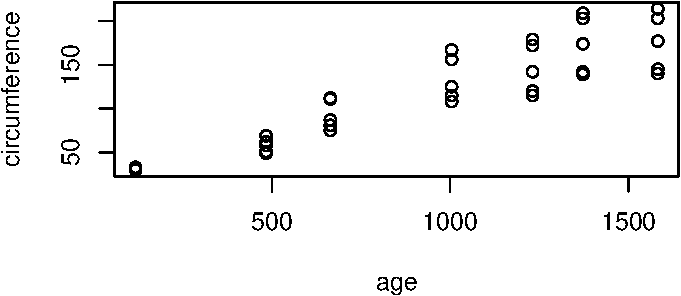
\includegraphics{03_introR02_files/figure-beamer/unnamed-chunk-16-1.pdf}

}

\end{figure}
\end{frame}

\begin{frame}[fragile]{2.7.2 Some elementary built-in functions}
\protect\hypertarget{some-elementary-built-in-functions}{}
\begin{block}{The sample median}
\protect\hypertarget{the-sample-median}{}
\begin{itemize}
\tightlist
\item
  The sample median measures the middle value of a data set. If the
  ordered data are \(x[1] \leq x[2] \leq \ldots \leq x[n]\), \[
  \text{median}(x) = 
  \begin{cases}
  x[(n + 1)/2], & n \text{ is odd}\\
  \{[x[n/2] + x[n/2 + 1]\}/2 & n \text{ is even}
  \end{cases}.
  \]
\end{itemize}

\begin{Shaded}
\begin{Highlighting}[]
\NormalTok{values\_1 }\OtherTok{\textless{}{-}} \FunctionTok{c}\NormalTok{(}\DecValTok{10}\NormalTok{, }\DecValTok{10}\NormalTok{, }\DecValTok{18}\NormalTok{, }\DecValTok{30}\NormalTok{, }\DecValTok{32}\NormalTok{)}
\FunctionTok{median}\NormalTok{(values\_1)}
\end{Highlighting}
\end{Shaded}

\begin{verbatim}
[1] 18
\end{verbatim}

\begin{Shaded}
\begin{Highlighting}[]
\NormalTok{values\_2 }\OtherTok{\textless{}{-}} \FunctionTok{c}\NormalTok{(}\DecValTok{40}\NormalTok{, }\DecValTok{10}\NormalTok{, }\DecValTok{10}\NormalTok{, }\DecValTok{18}\NormalTok{, }\DecValTok{30}\NormalTok{, }\DecValTok{32}\NormalTok{)}
\FunctionTok{median}\NormalTok{(values\_2) }\CommentTok{\#average of 18 and 30}
\end{Highlighting}
\end{Shaded}

\begin{verbatim}
[1] 24
\end{verbatim}
\end{block}
\end{frame}

\begin{frame}[fragile]
\begin{block}{Other summary measures}
\protect\hypertarget{other-summary-measures}{}
\begin{itemize}
\tightlist
\item
  Summary statistics can be calculated for data stored in vectors. In
  particular, try
\end{itemize}

\begin{Shaded}
\begin{Highlighting}[]
\FunctionTok{var}\NormalTok{(x) }\CommentTok{\# computes the variance of the data in x}
\FunctionTok{summary}\NormalTok{(x) }\CommentTok{\# computes several summary statistics on the data in x length(x) }
          \CommentTok{\# number of elements in x}
\FunctionTok{min}\NormalTok{(x) }\CommentTok{\# minimum value of x}
\FunctionTok{max}\NormalTok{(x) }\CommentTok{\# maximum value of x}
\FunctionTok{pmin}\NormalTok{(x, y) }\CommentTok{\# pairwise minima of corresponding elements of x and y pmax(x, y) }
          \CommentTok{\# pairwise maxima of x and y}
\FunctionTok{range}\NormalTok{(x) }\CommentTok{\# difference between maximum and minimum of data in x }
\FunctionTok{IQR}\NormalTok{(x) }\CommentTok{\# interquartile range: difference between 1st and 3rd}
        \CommentTok{\# quartiles of data in x}
\end{Highlighting}
\end{Shaded}

\begin{itemize}
\tightlist
\item
  For an example of the calculation of pairwise minima of two vectors,
  consider
\end{itemize}

\begin{Shaded}
\begin{Highlighting}[]
\NormalTok{x }\OtherTok{\textless{}{-}} \DecValTok{1}\SpecialCharTok{:}\DecValTok{5} 
\NormalTok{y }\OtherTok{\textless{}{-}} \DecValTok{7}\SpecialCharTok{:}\DecValTok{3} 
\FunctionTok{pmin}\NormalTok{(x,y)}
\end{Highlighting}
\end{Shaded}

\begin{verbatim}
[1] 1 2 3 4 3
\end{verbatim}
\end{block}
\end{frame}

\begin{frame}[fragile]{2.7.3 Presenting results using R Markdown}
\protect\hypertarget{presenting-results-using-r-markdown}{}
\begin{itemize}
\tightlist
\item
  \textbf{R Markdown} is one way to make presenting results easier.

  \begin{itemize}
  \tightlist
  \item
    It is a mixture of \textbf{Markdown}, a simple way to write a
    document in a plain text file, and \textbf{chunks} of code in R or
    another computer language.
  \item
    When you \textbf{render} the input into a document, R runs the code,
    automatically collects printed output and graphics and inserts them
    into the final document.
  \end{itemize}
\end{itemize}

\begin{itemize}
\item
  The simplest way to start is to ask RStudio to produce an initial
  template; then you delete the sample material, add your own, and
  render it. Using the menus in RStudio, choose
  \texttt{File\textbar{}New\ File\textbar{}R\ Markdown}\ldots.
\item
  You may choose an HTML document (a web page) or a PDF document.

  \begin{itemize}
  \tightlist
  \item
    In this template, the first part (between the two \texttt{-\/-\/-}
    lines) is called the \textbf{YAML}. It contains information that
    will be used when rendering your document.
  \item
    The actual document starts after the YAML. Headings are marked with
    an initial \texttt{\#\#}, and text is written out in an essentially
    normal way.
  \item
    Instructions within the template tell you how to include code chunks
    that will display results.
  \item
    To do the rendering, click on \texttt{Knit} in the top of the pane.
    This will ask to save the file if you haven't already done that,
    then render it and display the result on the screen.
  \end{itemize}
\end{itemize}
\end{frame}

\begin{frame}[fragile]{2.8 Logical vectors and relational operators}
\protect\hypertarget{logical-vectors-and-relational-operators}{}
\begin{block}{2.8.1 Boolean algebra}
\protect\hypertarget{boolean-algebra}{}
\begin{itemize}
\item
  The idea of \textbf{Boolean algebra} is to formalize a mathematical
  approach to logic. Logic deals with statements that are either true or
  false.
\item
  For example, let \(A\) is the statement that the sky is clear, and
  \(B\) is the statement that it is raining. Depending on the weather
  where you are,

  \begin{itemize}
  \item
    \begin{enumerate}
    [(1)]
    \tightlist
    \item
      those two statements may both be true (there is a
      \emph{sunshower}),
    \end{enumerate}
  \item
    \begin{enumerate}
    [(1)]
    \setcounter{enumi}{1}
    \tightlist
    \item
      \(A\) may be true and \(B\) false (the usual clear day),
    \end{enumerate}
  \item
    \begin{enumerate}
    [(1)]
    \setcounter{enumi}{2}
    \tightlist
    \item
      \(A\) false and \(B\) true (the usual rainy day), or
    \end{enumerate}
  \item
    \begin{enumerate}
    [(1)]
    \setcounter{enumi}{3}
    \tightlist
    \item
      both may be false (a cloudy but dry day).
    \end{enumerate}
  \end{itemize}
\end{itemize}

\begin{longtable}[]{@{}
  >{\centering\arraybackslash}p{(\columnwidth - 10\tabcolsep) * \real{0.1667}}
  >{\centering\arraybackslash}p{(\columnwidth - 10\tabcolsep) * \real{0.1667}}
  >{\centering\arraybackslash}p{(\columnwidth - 10\tabcolsep) * \real{0.1667}}
  >{\centering\arraybackslash}p{(\columnwidth - 10\tabcolsep) * \real{0.1667}}
  >{\centering\arraybackslash}p{(\columnwidth - 10\tabcolsep) * \real{0.1667}}
  >{\centering\arraybackslash}p{(\columnwidth - 10\tabcolsep) * \real{0.1667}}@{}}
\toprule\noalign{}
\begin{minipage}[b]{\linewidth}\centering
A\linebreak \texttt{A}
\end{minipage} & \begin{minipage}[b]{\linewidth}\centering
B\linebreak\texttt{B}
\end{minipage} & \begin{minipage}[b]{\linewidth}\centering
not A\linebreak\texttt{!A}
\end{minipage} & \begin{minipage}[b]{\linewidth}\centering
not B\linebreak\texttt{!B}
\end{minipage} & \begin{minipage}[b]{\linewidth}\centering
A and B\linebreak\texttt{A\ \&\ B}
\end{minipage} & \begin{minipage}[b]{\linewidth}\centering
A or B\linebreak\texttt{A\ \textbar{}\ B}
\end{minipage} \\
\midrule\noalign{}
\endhead
\texttt{TRUE} & \texttt{TRUE} & \texttt{FALSE} & \texttt{FALSE} &
\texttt{TRUE} & \texttt{TRUE} \\
\texttt{TRUE} & \texttt{FALSE} & \texttt{FALSE} & \texttt{TRUE} &
\texttt{FALSE} & \texttt{TRUE} \\
\texttt{FALSE} & \texttt{TRUE} & \texttt{TRUE} & \texttt{FALSE} &
\texttt{FALSE} & \texttt{TRUE} \\
\texttt{FALSE} & \texttt{FALSE} & \texttt{TRUE} & \texttt{TRUE} &
\texttt{FALSE} & \texttt{FALSE} \\
\bottomrule\noalign{}
\end{longtable}
\end{block}
\end{frame}

\begin{frame}[fragile]
\begin{block}{2.8.2 Logical operations in R}
\protect\hypertarget{logical-operations-in-r}{}
\begin{itemize}
\tightlist
\item
  A logical vector may be constructed as
\end{itemize}

\begin{Shaded}
\begin{Highlighting}[]
\NormalTok{a }\OtherTok{\textless{}{-}} \FunctionTok{c}\NormalTok{(}\ConstantTok{TRUE}\NormalTok{, }\ConstantTok{FALSE}\NormalTok{, }\ConstantTok{FALSE}\NormalTok{, }\ConstantTok{TRUE}\NormalTok{)}
\end{Highlighting}
\end{Shaded}

\begin{itemize}
\tightlist
\item
  Logical vectors may be used as indices. The elements of \texttt{b}
  corresponding to \texttt{TRUE} are selected.
\end{itemize}

\begin{Shaded}
\begin{Highlighting}[]
\NormalTok{b }\OtherTok{\textless{}{-}} \FunctionTok{c}\NormalTok{(}\DecValTok{13}\NormalTok{, }\DecValTok{7}\NormalTok{, }\DecValTok{8}\NormalTok{, }\DecValTok{2}\NormalTok{) }
\NormalTok{b[a]}
\end{Highlighting}
\end{Shaded}

\begin{verbatim}
[1] 13  2
\end{verbatim}

\begin{itemize}
\tightlist
\item
  If we attempt arithmetic on a logical vector, then the operations are
  performed after converting \texttt{FALSE} to \texttt{0} and
  \texttt{TRUE} to \texttt{1}.
\end{itemize}

\begin{Shaded}
\begin{Highlighting}[]
\FunctionTok{sum}\NormalTok{(a) }\CommentTok{\#we count how many occurrences of TRUE are in the vector.}
\end{Highlighting}
\end{Shaded}

\begin{verbatim}
[1] 2
\end{verbatim}

\begin{itemize}
\tightlist
\item
  There are two versions of the Boolean operators. The usual versions
  are \texttt{\&}, \texttt{\textbar{}} and \texttt{!}, as listed in the
  previous section. These are all vectorized.
\end{itemize}

\begin{Shaded}
\begin{Highlighting}[]
\SpecialCharTok{!}\NormalTok{a}
\end{Highlighting}
\end{Shaded}

\begin{verbatim}
[1] FALSE  TRUE  TRUE FALSE
\end{verbatim}
\end{block}
\end{frame}

\begin{frame}[fragile]
\begin{itemize}
\tightlist
\item
  If we attempt logical operations on a numerical vector, 0 is taken to
  be \texttt{FALSE}, and any non-zero value is taken to be
  \texttt{TRUE}:
\end{itemize}

\begin{Shaded}
\begin{Highlighting}[]
\NormalTok{a }\SpecialCharTok{\&}\NormalTok{ (b }\SpecialCharTok{{-}} \DecValTok{2}\NormalTok{)}
\end{Highlighting}
\end{Shaded}

\begin{verbatim}
[1]  TRUE FALSE FALSE FALSE
\end{verbatim}

\begin{itemize}
\tightlist
\item
  The operators \texttt{\&\&} and \texttt{\textbar{}\textbar{}} are
  similar to \texttt{\&} and \texttt{\textbar{}}, but behave differently
  in two respects.

  \begin{itemize}
  \tightlist
  \item
    First, they are not \textbf{vectorized}: only one calculation is
    done, and in newer versions of R, you'll get an error if you try to
    use them on longer vectors.
  \item
    Second, they are guaranteed to be evaluated from left to right, with
    the right-hand operand only evaluated if necessary.
  \end{itemize}
\end{itemize}

\begin{Shaded}
\begin{Highlighting}[]
\NormalTok{A }\OtherTok{\textless{}{-}} \ConstantTok{FALSE}\NormalTok{; B }\OtherTok{\textless{}{-}} \ConstantTok{TRUE}
\NormalTok{A }\SpecialCharTok{\&\&}\NormalTok{ B}
\end{Highlighting}
\end{Shaded}

\begin{verbatim}
[1] FALSE
\end{verbatim}

\begin{Shaded}
\begin{Highlighting}[]
\NormalTok{A }\OtherTok{\textless{}{-}} \ConstantTok{FALSE}\NormalTok{; B }\OtherTok{\textless{}{-}} \ConstantTok{FALSE}
\end{Highlighting}
\end{Shaded}

\begin{itemize}
\tightlist
\item
  This can save time if evaluating \texttt{B} would be very slow, and
  may make calculations easier, for example if evaluating \texttt{B}
  would cause an error when \texttt{A} was \texttt{FALSE}.
\end{itemize}
\end{frame}

\begin{frame}[fragile]
\begin{block}{2.8.3 Relational operators}
\protect\hypertarget{relational-operators}{}
\begin{itemize}
\tightlist
\item
  R allows the relational operators: \texttt{\textless{}},
  \texttt{\textgreater{}}, \texttt{==}, \texttt{\textgreater{}=},
  \texttt{\textless{}=}, \texttt{!=}.
\end{itemize}

\begin{Shaded}
\begin{Highlighting}[]
\NormalTok{threeM }\OtherTok{\textless{}{-}} \FunctionTok{c}\NormalTok{(}\DecValTok{3}\NormalTok{, }\DecValTok{6}\NormalTok{, }\DecValTok{9}\NormalTok{)}
\NormalTok{threeM }\SpecialCharTok{\textgreater{}} \DecValTok{4} \CommentTok{\# which elements are greater than 4}
\end{Highlighting}
\end{Shaded}

\begin{verbatim}
[1] FALSE  TRUE  TRUE
\end{verbatim}

\begin{Shaded}
\begin{Highlighting}[]
\NormalTok{threeM }\SpecialCharTok{==} \DecValTok{4}   \CommentTok{\# which elements are exactly equal to 4}
\end{Highlighting}
\end{Shaded}

\begin{verbatim}
[1] FALSE FALSE FALSE
\end{verbatim}

\begin{Shaded}
\begin{Highlighting}[]
\NormalTok{threeM }\SpecialCharTok{\textgreater{}=} \DecValTok{4}   \CommentTok{\# which elements are greater than or equal to 4}
\end{Highlighting}
\end{Shaded}

\begin{verbatim}
[1] FALSE  TRUE  TRUE
\end{verbatim}

\begin{Shaded}
\begin{Highlighting}[]
\NormalTok{threeM }\SpecialCharTok{!=} \DecValTok{4}   \CommentTok{\# which elements are not equal to 4}
\end{Highlighting}
\end{Shaded}

\begin{verbatim}
[1] TRUE TRUE TRUE
\end{verbatim}

\begin{Shaded}
\begin{Highlighting}[]
\NormalTok{threeM[threeM }\SpecialCharTok{\textgreater{}} \DecValTok{4}\NormalTok{] }\CommentTok{\# elements of threeM which are greater than 4}
\end{Highlighting}
\end{Shaded}

\begin{verbatim}
[1] 6 9
\end{verbatim}

\begin{Shaded}
\begin{Highlighting}[]
\NormalTok{four68 }\OtherTok{\textless{}{-}} \FunctionTok{c}\NormalTok{(}\DecValTok{4}\NormalTok{, }\DecValTok{6}\NormalTok{, }\DecValTok{8}\NormalTok{)}
\NormalTok{four68 }\SpecialCharTok{\textgreater{}}\NormalTok{ threeM }\CommentTok{\# four68 elements exceed corresponding threeM elements}
\end{Highlighting}
\end{Shaded}

\begin{verbatim}
[1]  TRUE FALSE FALSE
\end{verbatim}

\begin{Shaded}
\begin{Highlighting}[]
\NormalTok{four68[threeM }\SpecialCharTok{\textless{}}\NormalTok{ four68] }\CommentTok{\# print them}
\end{Highlighting}
\end{Shaded}

\begin{verbatim}
[1] 4
\end{verbatim}
\end{block}
\end{frame}

\begin{frame}[fragile]{2.9 Data frames, tibbles, and lists}
\protect\hypertarget{data-frames-tibbles-and-lists}{}
\begin{itemize}
\tightlist
\item
  Data sets frequently consist of more than one column of data, where +
  each column represents measurements of a single variable, and

  \begin{itemize}
  \tightlist
  \item
    each row usually represents a single observation.
  \end{itemize}
\item
  This format is referred to as \textbf{case-by-variable} format.
\end{itemize}

\begin{itemize}
\tightlist
\item
  Most data sets are stored in R as \texttt{data.frame}. An example is
  \texttt{women} which contains the average \texttt{height}s (in inches)
  and \texttt{weight}s (in pounds) of American women aged 30 to 39:
\end{itemize}

\begin{Shaded}
\begin{Highlighting}[]
\FunctionTok{head}\NormalTok{(women)}
\end{Highlighting}
\end{Shaded}

\begin{verbatim}
  height weight
1     58    115
2     59    117
3     60    120
4     61    123
5     62    126
6     63    129
\end{verbatim}
\end{frame}

\begin{frame}[fragile]
\begin{itemize}
\tightlist
\item
  Other ways to view the data are through the use of the
  \texttt{summary()} function as shown below, or by constructing an
  appropriate graph:
\end{itemize}

\begin{Shaded}
\begin{Highlighting}[]
\FunctionTok{summary}\NormalTok{(women)}
\end{Highlighting}
\end{Shaded}

\begin{verbatim}
     height         weight     
 Min.   :58.0   Min.   :115.0  
 1st Qu.:61.5   1st Qu.:124.5  
 Median :65.0   Median :135.0  
 Mean   :65.0   Mean   :136.7  
 3rd Qu.:68.5   3rd Qu.:148.0  
 Max.   :72.0   Max.   :164.0  
\end{verbatim}

\begin{Shaded}
\begin{Highlighting}[]
\FunctionTok{plot}\NormalTok{(weight }\SpecialCharTok{\textasciitilde{}}\NormalTok{ height, }\AttributeTok{data =}\NormalTok{ women)}
\end{Highlighting}
\end{Shaded}

\begin{figure}

{\centering 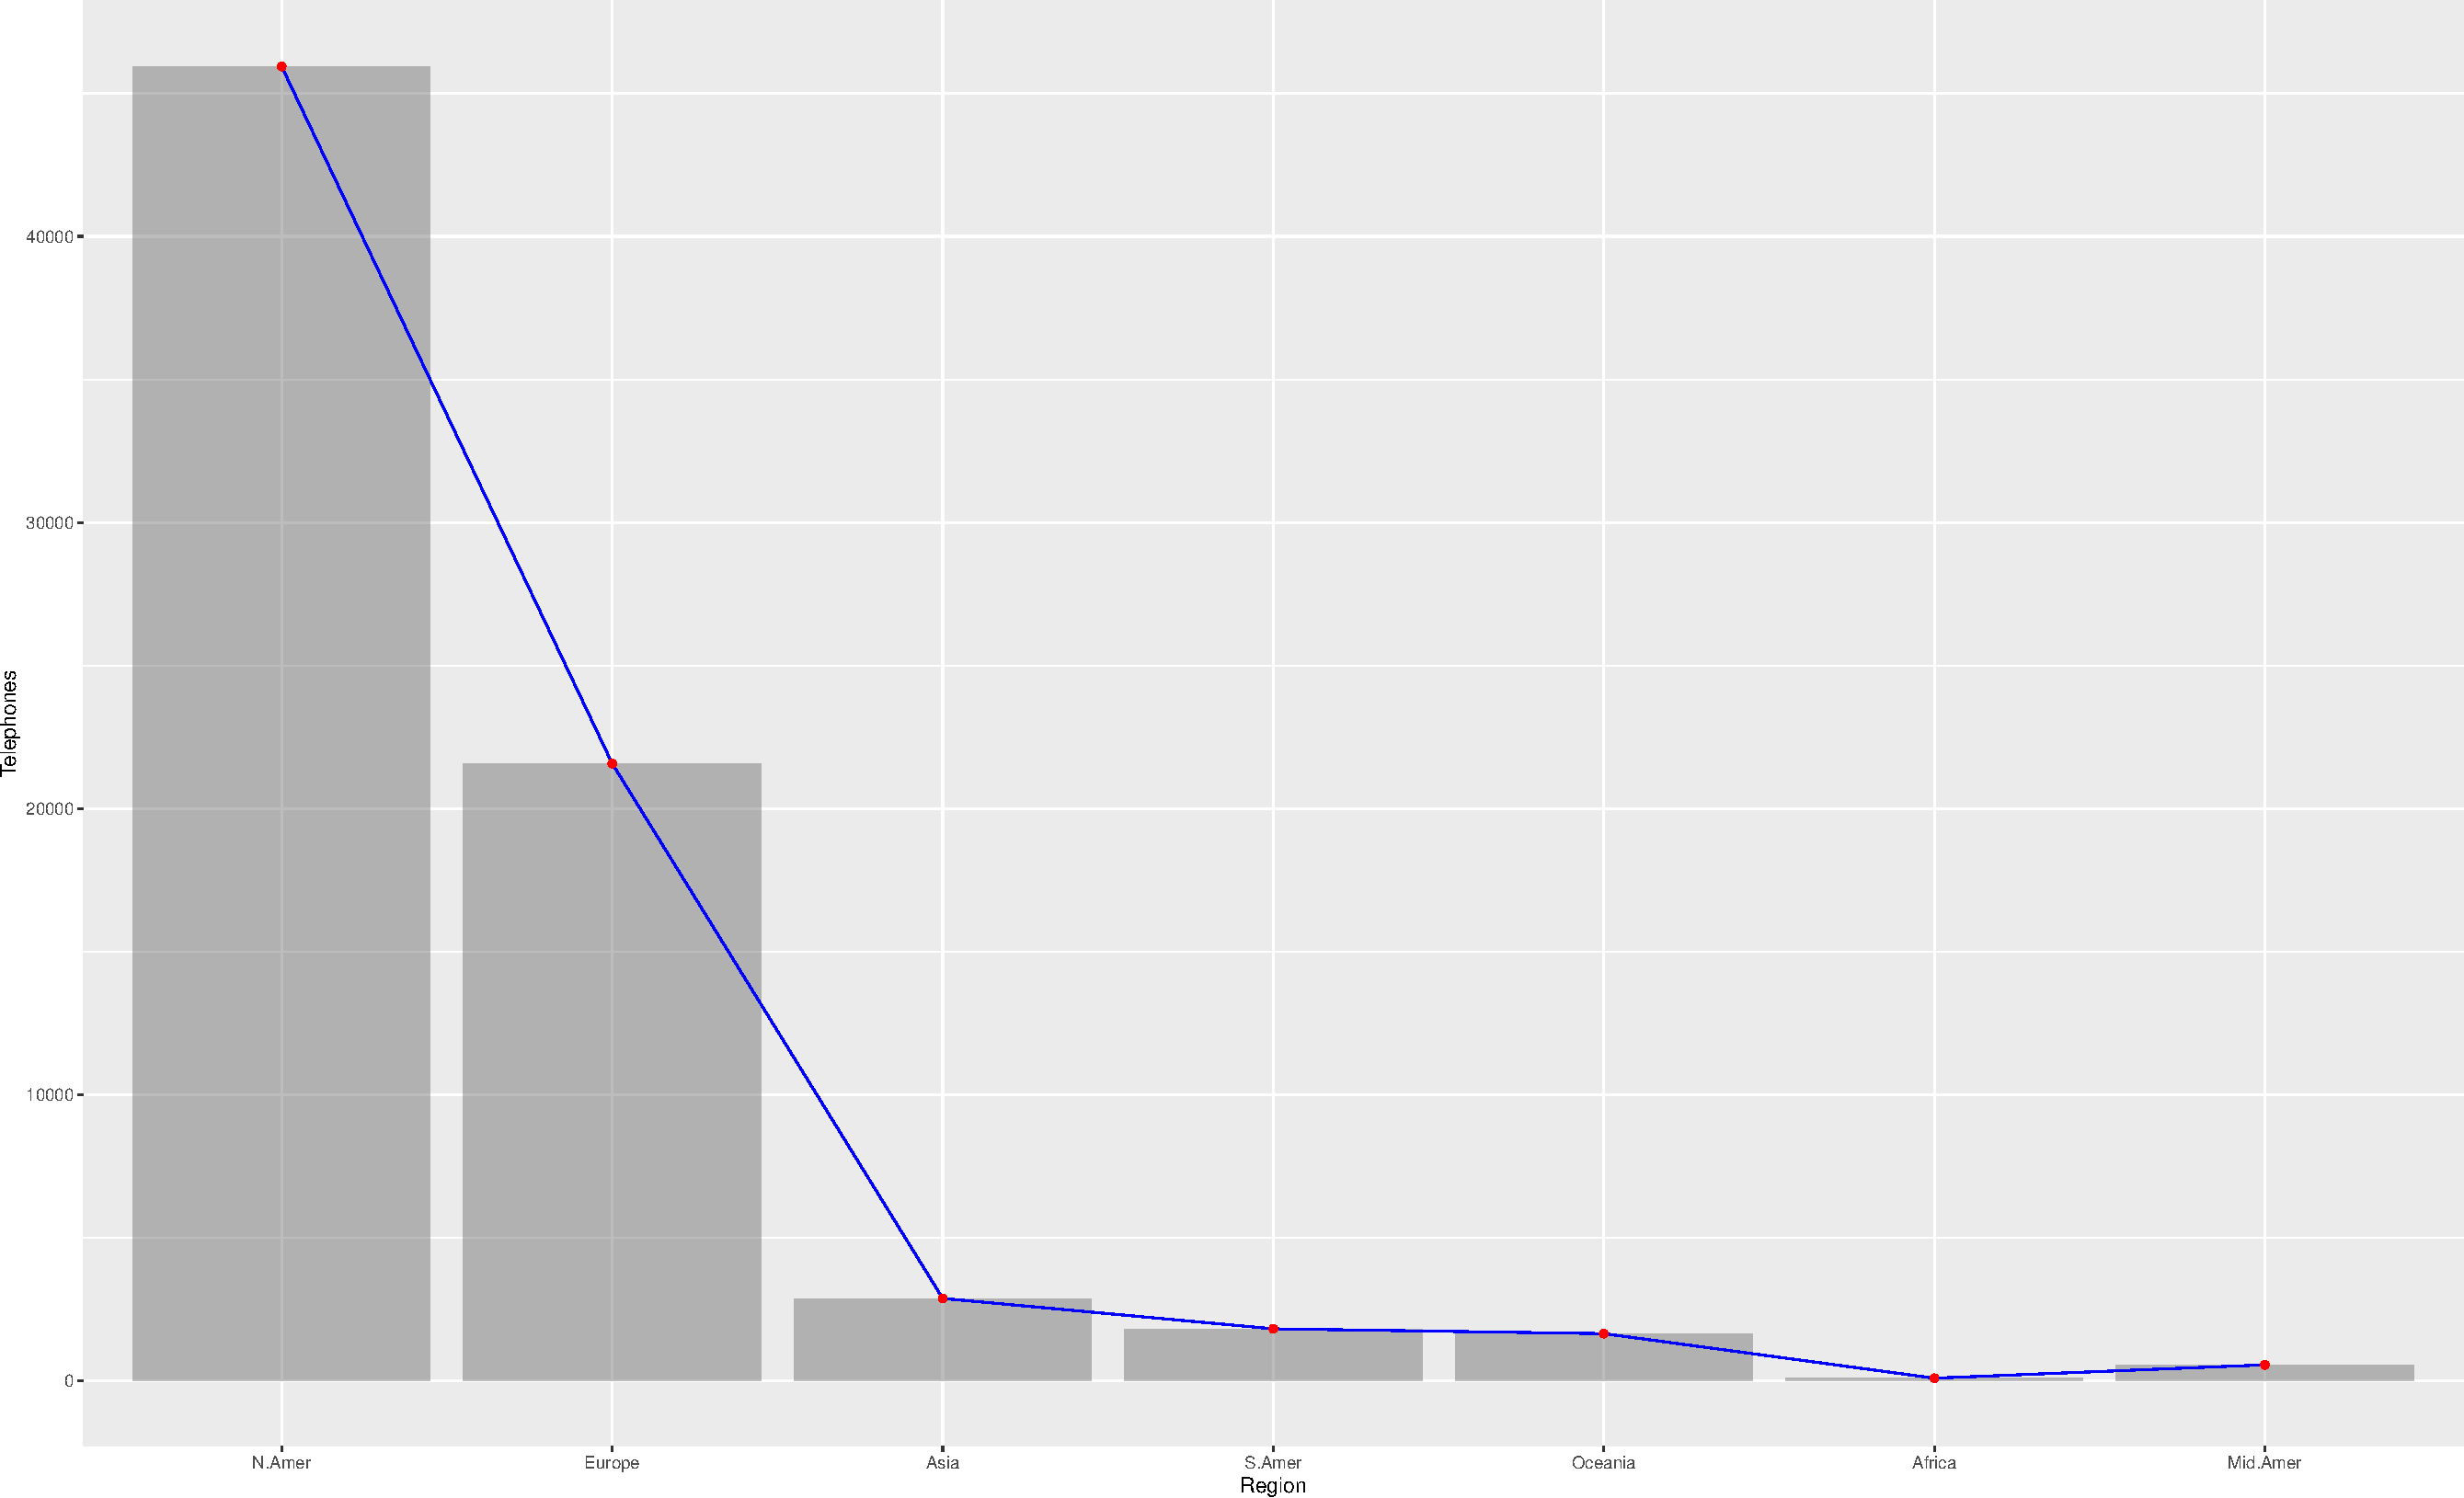
\includegraphics{03_introR02_files/figure-beamer/unnamed-chunk-28-1.pdf}

}

\end{figure}
\end{frame}

\begin{frame}[fragile]
\begin{itemize}
\tightlist
\item
  For larger data frames, a quick way of counting the number of rows and
  columns is important. The functions \texttt{nrow()} and
  \texttt{ncol()} play this role:
\end{itemize}

\begin{Shaded}
\begin{Highlighting}[]
\FunctionTok{nrow}\NormalTok{(women)}
\end{Highlighting}
\end{Shaded}

\begin{verbatim}
[1] 15
\end{verbatim}

\begin{Shaded}
\begin{Highlighting}[]
\FunctionTok{ncol}\NormalTok{(women)}
\end{Highlighting}
\end{Shaded}

\begin{verbatim}
[1] 2
\end{verbatim}

\begin{itemize}
\tightlist
\item
  We can get both at once using \texttt{dim()} (for dimension) and can
  get summary information using \texttt{str()} (for structure):
\end{itemize}

\begin{Shaded}
\begin{Highlighting}[]
\FunctionTok{dim}\NormalTok{(women)}
\end{Highlighting}
\end{Shaded}

\begin{verbatim}
[1] 15  2
\end{verbatim}

\begin{Shaded}
\begin{Highlighting}[]
\FunctionTok{str}\NormalTok{(women)}
\end{Highlighting}
\end{Shaded}

\begin{verbatim}
'data.frame':   15 obs. of  2 variables:
 $ height: num  58 59 60 61 62 63 64 65 66 67 ...
 $ weight: num  115 117 120 123 126 129 132 135 139 142 ...
\end{verbatim}

\begin{itemize}
\tightlist
\item
  In fact, \texttt{str()} works with almost any R object, and is often a
  quick way to find what you are working with.
\end{itemize}
\end{frame}

\begin{frame}[fragile]
\begin{block}{2.9.1 Extracting data frame elements and subsets}
\protect\hypertarget{extracting-data-frame-elements-and-subsets}{}
\begin{itemize}
\tightlist
\item
  We can extract elements from data frames using similar syntax to what
  was used with matrices.
\end{itemize}

\begin{Shaded}
\begin{Highlighting}[]
\NormalTok{women[}\DecValTok{7}\NormalTok{, }\DecValTok{2}\NormalTok{]}
\end{Highlighting}
\end{Shaded}

\begin{verbatim}
[1] 132
\end{verbatim}

\begin{Shaded}
\begin{Highlighting}[]
\CommentTok{\#try at home}
\CommentTok{\#women[3, ]; women[4:7, 1]}
\end{Highlighting}
\end{Shaded}

\begin{itemize}
\tightlist
\item
  Data frame columns can also be addressed using their names using the
  \texttt{\$} operator. For example, the weight column can be extracted
  as follows:
\end{itemize}

\begin{Shaded}
\begin{Highlighting}[]
\NormalTok{women}\SpecialCharTok{$}\NormalTok{weight}
\end{Highlighting}
\end{Shaded}

\begin{verbatim}
 [1] 115 117 120 123 126 129 132 135 139 142 146 150 154 159 164
\end{verbatim}

\begin{itemize}
\tightlist
\item
  Thus, we can extract all heights for which the weights exceed 140
  using
\end{itemize}

\begin{Shaded}
\begin{Highlighting}[]
\NormalTok{women}\SpecialCharTok{$}\NormalTok{height[women}\SpecialCharTok{$}\NormalTok{weight }\SpecialCharTok{\textgreater{}} \DecValTok{140}\NormalTok{]}
\end{Highlighting}
\end{Shaded}

\begin{verbatim}
[1] 67 68 69 70 71 72
\end{verbatim}

\begin{itemize}
\tightlist
\item
  The \texttt{with()} function allows us to access columns of a
  \texttt{data.frame} directly without using the \texttt{\$}.
\end{itemize}

\begin{Shaded}
\begin{Highlighting}[]
\FunctionTok{with}\NormalTok{(women, weight}\SpecialCharTok{/}\NormalTok{height)}
\end{Highlighting}
\end{Shaded}

\begin{verbatim}
 [1] 1.982759 1.983051 2.000000 2.016393 2.032258 2.047619 2.062500 2.076923
 [9] 2.106061 2.119403 2.147059 2.173913 2.200000 2.239437 2.277778
\end{verbatim}
\end{block}
\end{frame}

\begin{frame}[fragile]
\begin{block}{2.9.2 Taking random samples from populations}
\protect\hypertarget{taking-random-samples-from-populations}{}
\begin{itemize}
\tightlist
\item
  The \texttt{sample()} function can be used to take samples (with or
  without replacement) from larger finite populations.
\end{itemize}

\begin{itemize}
\tightlist
\item
  Suppose that we have a data consisting of 15000 entries, and we would
  like to randomly select 8 entries (without replacement) for detailed
  study. It can be realized by selecting a random sample of indices:
\end{itemize}

\begin{Shaded}
\begin{Highlighting}[]
\NormalTok{sampleID }\OtherTok{\textless{}{-}} \FunctionTok{sample}\NormalTok{(}\DecValTok{1}\SpecialCharTok{:}\DecValTok{15000}\NormalTok{, }\AttributeTok{size =} \DecValTok{8}\NormalTok{, }\AttributeTok{replace =} \ConstantTok{FALSE}\NormalTok{) }
\NormalTok{sampleID}
\end{Highlighting}
\end{Shaded}

\begin{verbatim}
[1] 11759   904   776   654  2803 12814   713   497
\end{verbatim}
\end{block}
\end{frame}

\begin{frame}[fragile]
\begin{block}{2.9.3 Constructing data frames}
\protect\hypertarget{constructing-data-frames}{}
\begin{itemize}
\tightlist
\item
  Use the \texttt{data.frame()} function to construct data frames from
  vectors that already exist in your workspace:
\end{itemize}

\begin{Shaded}
\begin{Highlighting}[]
\NormalTok{xy }\OtherTok{\textless{}{-}} \FunctionTok{data.frame}\NormalTok{(x, y)}
\NormalTok{xy}
\end{Highlighting}
\end{Shaded}

\begin{verbatim}
  x y
1 1 7
2 2 6
3 3 5
4 4 4
5 5 3
\end{verbatim}

\begin{itemize}
\tightlist
\item
  For another example, consider
\end{itemize}

\begin{Shaded}
\begin{Highlighting}[]
\NormalTok{xynew }\OtherTok{\textless{}{-}} \FunctionTok{data.frame}\NormalTok{(x, y, }\AttributeTok{new =} \DecValTok{10}\SpecialCharTok{:}\DecValTok{1}\NormalTok{)}
\end{Highlighting}
\end{Shaded}
\end{block}
\end{frame}

\begin{frame}[fragile]
\begin{block}{2.9.4 Data frames can have non-numeric columns}
\protect\hypertarget{data-frames-can-have-non-numeric-columns}{}
\begin{itemize}
\tightlist
\item
  Columns of data frames can be of different types. For example, the
  built-in data frame \texttt{chickwts} has a numeric column and a
  factor. Again, the \texttt{summary()} function provides a quick peek
  at this data set.
\end{itemize}

\begin{Shaded}
\begin{Highlighting}[]
\FunctionTok{summary}\NormalTok{(chickwts)}
\end{Highlighting}
\end{Shaded}

\begin{verbatim}
     weight             feed   
 Min.   :108.0   casein   :12  
 1st Qu.:204.5   horsebean:10  
 Median :258.0   linseed  :12  
 Mean   :261.3   meatmeal :11  
 3rd Qu.:323.5   soybean  :14  
 Max.   :423.0   sunflower:12  
\end{verbatim}

\begin{itemize}
\tightlist
\item
  Here, displaying the entire data frame would have been a waste of
  space, as can be seen from:
\end{itemize}

\begin{Shaded}
\begin{Highlighting}[]
\FunctionTok{nrow}\NormalTok{(chickwts)}
\end{Highlighting}
\end{Shaded}

\begin{verbatim}
[1] 71
\end{verbatim}
\end{block}
\end{frame}

\begin{frame}[fragile]
\begin{itemize}
\tightlist
\item
  An important point to be aware of is that in older versions of R
  (before 4.0.0), the \texttt{data.frame()} function automatically
  converted character vectors to factors. As an example, consider the
  following data that might be used as a baseline in an obesity study:
\end{itemize}

\begin{Shaded}
\begin{Highlighting}[]
\NormalTok{gender }\OtherTok{\textless{}{-}} \FunctionTok{c}\NormalTok{(}\StringTok{"M"}\NormalTok{, }\StringTok{"M"}\NormalTok{, }\StringTok{"F"}\NormalTok{, }\StringTok{"F"}\NormalTok{, }\StringTok{"F"}\NormalTok{) }
\NormalTok{weight }\OtherTok{\textless{}{-}} \FunctionTok{c}\NormalTok{(}\DecValTok{73}\NormalTok{, }\DecValTok{68}\NormalTok{, }\DecValTok{52}\NormalTok{, }\DecValTok{69}\NormalTok{, }\DecValTok{64}\NormalTok{) }
\NormalTok{obesityStudy }\OtherTok{\textless{}{-}} \FunctionTok{data.frame}\NormalTok{(gender, weight)}
\end{Highlighting}
\end{Shaded}

\begin{itemize}
\tightlist
\item
  The vector \texttt{gender} is clearly a character vector, and in R
  4.0.0 or later it will be left that way in the data frame:
\end{itemize}

\begin{Shaded}
\begin{Highlighting}[]
\NormalTok{obesityStudy}\SpecialCharTok{$}\NormalTok{gender}
\end{Highlighting}
\end{Shaded}

\begin{verbatim}
[1] "M" "M" "F" "F" "F"
\end{verbatim}

\begin{itemize}
\tightlist
\item
  If you want the older behavior, use the
  \texttt{stringsAsFactors\ =\ TRUE} argument when you create the data
  frame:
\end{itemize}

\begin{Shaded}
\begin{Highlighting}[]
\NormalTok{obesityStudy }\OtherTok{\textless{}{-}} \FunctionTok{data.frame}\NormalTok{(gender, weight, }\AttributeTok{stringsAsFactors =} \ConstantTok{TRUE}\NormalTok{) }
\NormalTok{obesityStudy}\SpecialCharTok{$}\NormalTok{gender}
\end{Highlighting}
\end{Shaded}

\begin{verbatim}
[1] M M F F F
Levels: F M
\end{verbatim}
\end{frame}

\begin{frame}[fragile]
\begin{itemize}
\tightlist
\item
  Now, suppose we wish to globally change \texttt{F} to \texttt{Female}
  in the data frame. An incorrect approach is
\end{itemize}

\begin{Shaded}
\begin{Highlighting}[]
\NormalTok{wrongWay }\OtherTok{\textless{}{-}}\NormalTok{ obesityStudy}
\NormalTok{whereF }\OtherTok{\textless{}{-}}\NormalTok{ wrongWay}\SpecialCharTok{$}\NormalTok{gender }\SpecialCharTok{==} \StringTok{"F"}
\NormalTok{wrongWay}\SpecialCharTok{$}\NormalTok{gender[whereF] }\OtherTok{\textless{}{-}} \StringTok{"Female"}
\end{Highlighting}
\end{Shaded}

\begin{verbatim}
Warning in `[<-.factor`(`*tmp*`, whereF, value = structure(c(2L, 2L, NA, :
invalid factor level, NA generated
\end{verbatim}

\begin{Shaded}
\begin{Highlighting}[]
\NormalTok{wrongWay}\SpecialCharTok{$}\NormalTok{gender}
\end{Highlighting}
\end{Shaded}

\begin{verbatim}
[1] M    M    <NA> <NA> <NA>
Levels: F M
\end{verbatim}

\begin{itemize}
\tightlist
\item
  The correct approach is through the levels of the
  \texttt{obesityStudy\$gender} factor:
\end{itemize}

\begin{Shaded}
\begin{Highlighting}[]
\FunctionTok{levels}\NormalTok{(obesityStudy}\SpecialCharTok{$}\NormalTok{gender)[}\DecValTok{1}\NormalTok{] }\OtherTok{\textless{}{-}} \StringTok{"Female"} \CommentTok{\# F is the 1st level {-}{-} why? }
\NormalTok{obesityStudy}\SpecialCharTok{$}\NormalTok{gender }\CommentTok{\# check that F was really replaced by Female}
\end{Highlighting}
\end{Shaded}

\begin{verbatim}
[1] M      M      Female Female Female
Levels: Female M
\end{verbatim}
\end{frame}

\begin{frame}[fragile]
\begin{block}{2.9.5 Lists}
\protect\hypertarget{lists}{}
\begin{itemize}
\tightlist
\item
  Data frames are actually a special kind of \textbf{list}, or
  structure. Lists in R can contain any other objects.
\end{itemize}

\begin{itemize}
\tightlist
\item
  The \texttt{list()} function is one way of organizing multiple pieces
  of output from functions. For example,
\end{itemize}

\begin{Shaded}
\begin{Highlighting}[]
\NormalTok{x }\OtherTok{\textless{}{-}} \FunctionTok{c}\NormalTok{(}\DecValTok{3}\NormalTok{, }\DecValTok{2}\NormalTok{, }\DecValTok{3}\NormalTok{)}
\NormalTok{y }\OtherTok{\textless{}{-}} \FunctionTok{c}\NormalTok{(}\DecValTok{7}\NormalTok{, }\DecValTok{7}\NormalTok{)}
\NormalTok{z }\OtherTok{\textless{}{-}} \FunctionTok{list}\NormalTok{(}\AttributeTok{x =}\NormalTok{ x, }\AttributeTok{y =}\NormalTok{ y) }
\NormalTok{z}
\end{Highlighting}
\end{Shaded}

\begin{verbatim}
$x
[1] 3 2 3

$y
[1] 7 7
\end{verbatim}
\end{block}
\end{frame}

\begin{frame}[fragile]
\begin{itemize}
\tightlist
\item
  You can see the names of the objects in a list using the
  \texttt{names()} function, and extract parts of it:
\end{itemize}

\begin{Shaded}
\begin{Highlighting}[]
\FunctionTok{names}\NormalTok{(z) }\CommentTok{\# Print names of objects in list z}
\end{Highlighting}
\end{Shaded}

\begin{verbatim}
[1] "x" "y"
\end{verbatim}

\begin{Shaded}
\begin{Highlighting}[]
\NormalTok{z}\SpecialCharTok{$}\NormalTok{x }\CommentTok{\# Print the x component of z}
\end{Highlighting}
\end{Shaded}

\begin{verbatim}
[1] 3 2 3
\end{verbatim}

\begin{itemize}
\tightlist
\item
  There are several functions which make working with lists easy. Two of
  them are \texttt{lapply()} and \texttt{vapply()}. The
  \texttt{lapply()} function \textbf{applies} another function to every
  element of a list and returns the results in a new list.
\end{itemize}

\begin{Shaded}
\begin{Highlighting}[]
\FunctionTok{lapply}\NormalTok{(z, mean)}
\end{Highlighting}
\end{Shaded}

\begin{verbatim}
$x
[1] 2.666667

$y
[1] 7
\end{verbatim}
\end{frame}

\begin{frame}[fragile]
\begin{itemize}
\tightlist
\item
  Sometimes it might be more convenient to have the results in a vector;
  the \texttt{vapply()} function does that.
\end{itemize}

\begin{Shaded}
\begin{Highlighting}[]
\FunctionTok{vapply}\NormalTok{(z, mean, }\DecValTok{1}\NormalTok{)}
\end{Highlighting}
\end{Shaded}

\begin{verbatim}
       x        y 
2.666667 7.000000 
\end{verbatim}

\begin{itemize}
\tightlist
\item
  If \texttt{mean()} had returned a different kind of result,
  \texttt{vapply()} would have given an error. If we expect more than a
  single value, the results will be organized into a matrix, e.g.
\end{itemize}

\begin{Shaded}
\begin{Highlighting}[]
\FunctionTok{vapply}\NormalTok{(z, summary, }\FunctionTok{numeric}\NormalTok{(}\DecValTok{6}\NormalTok{))}
\end{Highlighting}
\end{Shaded}

\begin{verbatim}
               x y
Min.    2.000000 7
1st Qu. 2.500000 7
Median  3.000000 7
Mean    2.666667 7
3rd Qu. 3.000000 7
Max.    3.000000 7
\end{verbatim}
\end{frame}

\begin{frame}[fragile]{2.10 Data input and output}
\protect\hypertarget{data-input-and-output}{}
\begin{block}{2.10.1 Changing directories}
\protect\hypertarget{changing-directories}{}
\begin{itemize}
\tightlist
\item
  In the RStudio Files Pane you can navigate to the directory where you
  want to work, and choose Set \texttt{As\ Working\ Directory} from the
  \texttt{More} menu item.
\end{itemize}

\begin{figure}

{\centering 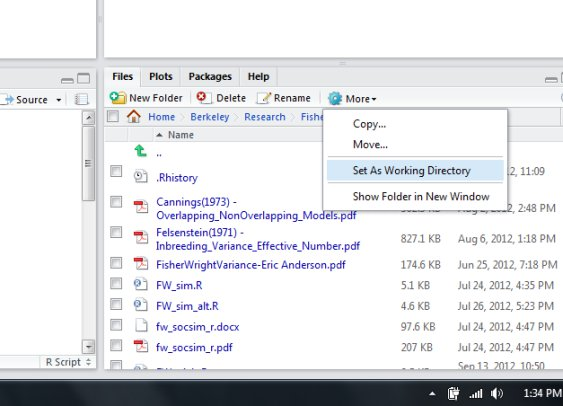
\includegraphics[width=0.4\textwidth,height=\textheight]{images/setasworkingdirectory.jpeg}

}

\caption{You can use File tab to change the working directory.}

\end{figure}

\begin{itemize}
\tightlist
\item
  Alternatively you can run the R function \texttt{setwd()}. For
  example, to work with data in the folder mydata on the C: drive, run
\end{itemize}

\begin{Shaded}
\begin{Highlighting}[]
\FunctionTok{setwd}\NormalTok{(}\StringTok{"c:/mydata"}\NormalTok{) }\CommentTok{\# or setwd("c:\textbackslash{}\textbackslash{}mydata") \#example: for WINDOWS}
\FunctionTok{setwd}\NormalTok{(}\StringTok{"\textasciitilde{}/Desktops/mydata"}\NormalTok{) }\CommentTok{\#example: for MAC OS}
\end{Highlighting}
\end{Shaded}
\end{block}
\end{frame}

\begin{frame}[fragile]
\begin{block}{2.10.2 \texttt{dump()} and \texttt{source()}}
\protect\hypertarget{dump-and-source}{}
\begin{itemize}
\tightlist
\item
  Suppose you have constructed an R object called \texttt{usefuldata}.
  In order to save this object for a future session, type
\end{itemize}

\begin{Shaded}
\begin{Highlighting}[]
\FunctionTok{dump}\NormalTok{(}\StringTok{"usefuldata"}\NormalTok{, }\StringTok{"useful.R"}\NormalTok{)}
\end{Highlighting}
\end{Shaded}

This stores the command necessary to create the vector
\texttt{usefuldata} into the file \texttt{useful.R} on your computer's
hard drive. The choice of filename is up to you, as long as it conforms
to the usual requirements for filenames on your computer.

\begin{itemize}
\tightlist
\item
  To retrieve the vector in a future session, type
\end{itemize}

\begin{Shaded}
\begin{Highlighting}[]
\FunctionTok{dump}\NormalTok{(}\AttributeTok{list =} \FunctionTok{objects}\NormalTok{(), }\StringTok{"all.R"}\NormalTok{)}
\end{Highlighting}
\end{Shaded}

This produces a file called \texttt{all.R} on your computer's hard
drive. Using \texttt{source("all.R")} at a later time will allow you to
retrieve all of these objects.
\end{block}

\begin{block}{Example 2.4}
\protect\hypertarget{example-2.4}{}
To save existing objects \texttt{humidity}, \texttt{temp} and
\texttt{rain} to a file called \texttt{weather.R} on your hard drive,
type

\begin{Shaded}
\begin{Highlighting}[]
\FunctionTok{dump}\NormalTok{(}\FunctionTok{c}\NormalTok{(}\StringTok{"humidity"}\NormalTok{, }\StringTok{"temp"}\NormalTok{, }\StringTok{"rain"}\NormalTok{), }\StringTok{"weather.R"}\NormalTok{)}
\end{Highlighting}
\end{Shaded}
\end{block}
\end{frame}



\end{document}
